\documentclass[man]{apa6}
\usepackage{lmodern}
\usepackage{amssymb,amsmath}
\usepackage{ifxetex,ifluatex}
\usepackage{fixltx2e} % provides \textsubscript
\ifnum 0\ifxetex 1\fi\ifluatex 1\fi=0 % if pdftex
  \usepackage[T1]{fontenc}
  \usepackage[utf8]{inputenc}
\else % if luatex or xelatex
  \ifxetex
    \usepackage{mathspec}
  \else
    \usepackage{fontspec}
  \fi
  \defaultfontfeatures{Ligatures=TeX,Scale=MatchLowercase}
\fi
% use upquote if available, for straight quotes in verbatim environments
\IfFileExists{upquote.sty}{\usepackage{upquote}}{}
% use microtype if available
\IfFileExists{microtype.sty}{%
\usepackage{microtype}
\UseMicrotypeSet[protrusion]{basicmath} % disable protrusion for tt fonts
}{}
\usepackage{hyperref}
\hypersetup{unicode=true,
            pdftitle={The Distinct Social Function of Disgust and Anger in the Moral Domain},
            pdfauthor={Jeffrey Kravitz},
            pdfkeywords={morality, character, anger, disgust},
            pdfborder={0 0 0},
            breaklinks=true}
\urlstyle{same}  % don't use monospace font for urls
\usepackage{graphicx,grffile}
\makeatletter
\def\maxwidth{\ifdim\Gin@nat@width>\linewidth\linewidth\else\Gin@nat@width\fi}
\def\maxheight{\ifdim\Gin@nat@height>\textheight\textheight\else\Gin@nat@height\fi}
\makeatother
% Scale images if necessary, so that they will not overflow the page
% margins by default, and it is still possible to overwrite the defaults
% using explicit options in \includegraphics[width, height, ...]{}
\setkeys{Gin}{width=\maxwidth,height=\maxheight,keepaspectratio}
\IfFileExists{parskip.sty}{%
\usepackage{parskip}
}{% else
\setlength{\parindent}{0pt}
\setlength{\parskip}{6pt plus 2pt minus 1pt}
}
\setlength{\emergencystretch}{3em}  % prevent overfull lines
\providecommand{\tightlist}{%
  \setlength{\itemsep}{0pt}\setlength{\parskip}{0pt}}
\setcounter{secnumdepth}{0}
% Redefines (sub)paragraphs to behave more like sections
\ifx\paragraph\undefined\else
\let\oldparagraph\paragraph
\renewcommand{\paragraph}[1]{\oldparagraph{#1}\mbox{}}
\fi
\ifx\subparagraph\undefined\else
\let\oldsubparagraph\subparagraph
\renewcommand{\subparagraph}[1]{\oldsubparagraph{#1}\mbox{}}
\fi

%%% Use protect on footnotes to avoid problems with footnotes in titles
\let\rmarkdownfootnote\footnote%
\def\footnote{\protect\rmarkdownfootnote}


  \title{The Distinct Social Function of Disgust and Anger in the Moral Domain}
    \author{Jeffrey Kravitz\textsuperscript{ }}
    \date{}
  
\shorttitle{SOCIAL FUNCTION OF DISGUST AND ANGER}
\affiliation{
\vspace{0.5cm}
\textsuperscript{ } CUNY Brooklyn College}
\keywords{morality, character, anger, disgust\newline\indent Word count:  }
\usepackage{csquotes}
\usepackage{upgreek}
\captionsetup{font=singlespacing,justification=justified}

\usepackage{longtable}
\usepackage{lscape}
\usepackage{multirow}
\usepackage{tabularx}
\usepackage[flushleft]{threeparttable}
\usepackage{threeparttablex}

\newenvironment{lltable}{\begin{landscape}\begin{center}\begin{ThreePartTable}}{\end{ThreePartTable}\end{center}\end{landscape}}

\makeatletter
\newcommand\LastLTentrywidth{1em}
\newlength\longtablewidth
\setlength{\longtablewidth}{1in}
\newcommand{\getlongtablewidth}{\begingroup \ifcsname LT@\roman{LT@tables}\endcsname \global\longtablewidth=0pt \renewcommand{\LT@entry}[2]{\global\advance\longtablewidth by ##2\relax\gdef\LastLTentrywidth{##2}}\@nameuse{LT@\roman{LT@tables}} \fi \endgroup}


\DeclareDelayedFloatFlavor{ThreePartTable}{table}
\DeclareDelayedFloatFlavor{lltable}{table}
\DeclareDelayedFloatFlavor*{longtable}{table}
\makeatletter
\renewcommand{\efloat@iwrite}[1]{\immediate\expandafter\protected@write\csname efloat@post#1\endcsname{}}
\makeatother

\authornote{

Correspondence concerning this article should be addressed to Jeffrey
Kravitz, N/A. E-mail:
\href{mailto:jkravitz.edu@gmail.com}{\nolinkurl{jkravitz.edu@gmail.com}}}

\abstract{
Recent research has drawn a distinction between moral judgments directly
focused on a transgressor's act and judgments focused on a
transgressor's character. Functional-evolutionary theories of emotion
posit that bad character should elicit disgust (a withdrawal emotion)
because stable, negative traits are unlikely to change, so the best
course of action may be to avoid those with bad character. By contrast,
the transgressions themselves should elicit anger (an approach emotion),
which may serve to change the transgressor's future behavior. The
current study aimed to provide further evidence for these hypotheses by
manipulating a transgressor's character and testing how this affects
feelings of disgust and anger. To manipulate character, we provided
information about the transgressor' prior good deeds, compared to a
control condition in which no positive information was provided.
Participants rated the transgressor's character and the wrongness of
their act, and also reported on disgust and anger.


}

\begin{document}
\maketitle

Recent research has drawn a distinction between moral judgments directly
focused on a transgressor's act and judgments focused on a
transgressor's character (Uhlmann, Pizarro, \& Diermeier, 2015).
Functional-evolutionary theories of emotion posit that bad character
should elicit disgust (a withdrawal emotion) because stable, negative
traits are unlikely to change, so the best course of action may be to
avoid those with bad character. By contrast, the transgressions
themselves should elicit anger (an approach emotion), which may serve to
change the transgressor's future behavior (Giner-Sorolla \& Chapman,
2017). The current study aimed to provide further evidence for these
hypotheses by manipulating a transgressor's character and testing how
this affects feelings of disgust and anger.

\section{Methods}\label{methods}

In order to test this hypothesis, 212 participants sampled from Amazon's
Mechanical Turk completed an online survey programmed using Qualtrics
software. All participants read a fabricated \enquote{news artcle}
describing a high school principal who either sexually harassed a
waitress or was pulled over by a cop for using cocaine
(counterbalanced). To manipulate moral character of a transgessor, one
independent variable of Domain (Different vs.~Control vs.~Same) was
used. Participants in the \enquote{Different Domain} condition first
read a fabricated \enquote{news article} that described the principal's
benevolant actions in a domain other than that in which he transgressed
(e.g., a principal who campaigned against drug use was caught harassing
a woman, and vise versa). Participants in the \enquote{Same Domain}
condition first read a fabricated \enquote{news article} that described
the principal's benevolant actions in the same domain in which he
transgressed (e.g., a principal who campaigned against drug use was
pulled over for using cocaine, and vise versa). Participants in the
\enquote{Control} condition did not read any article about the
principal's benevolant actions. The principal who committed a
transgression in a different domain should be rated as having better
character than the principal who did not have any benevolant actions
(control). The principal who committed a trangression in the same domain
should have worse character than principal who did not have any
benevolant actions (control) due to the added effect of hypocrisy.

Participants completed measures on 6 dependent variables: (1) Act
Judgments of the principal, (2) Character Judgments of the principal,
(3) Emotion towards the principal in endorsements of words, (4) Emotion
towards the principal in endorsement of photographed faces, (5)
Hypocrisy Judgments of the principal, and (6) Disgust-Scale Ratings.

\section{Results}\label{results}

\begin{figure}
\centering
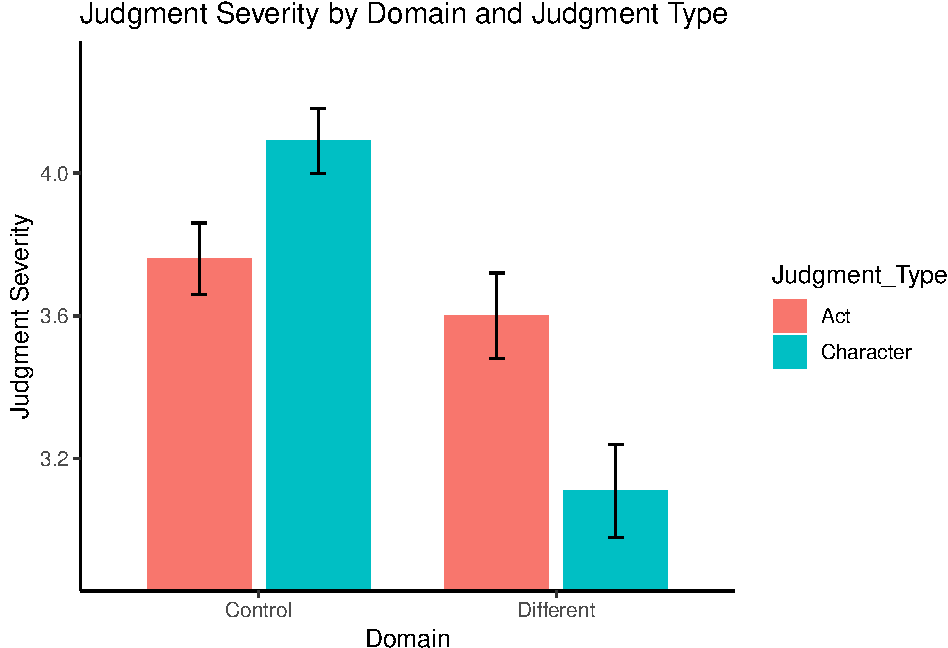
\includegraphics{APA_Report_files/figure-latex/unnamed-chunk-2-1.pdf}
\caption{\label{fig:unnamed-chunk-2}Severity of Act and Character judgments
by factor of Domain.}
\end{figure}

\begin{table}[tbp]
\begin{center}
\begin{threeparttable}
\caption{\label{tab:unnamed-chunk-3}ANOVA table for Hypothesis 1}
\begin{tabular}{lllllll}
\toprule
Effect & \multicolumn{1}{c}{$F$} & \multicolumn{1}{c}{$\mathit{df}_1$} & \multicolumn{1}{c}{$\mathit{df}_2$} & \multicolumn{1}{c}{$\mathit{MSE}$} & \multicolumn{1}{c}{$p$} & \multicolumn{1}{c}{$\hat{\eta}^2_G$}\\
\midrule
Domain & 17.37 & 1 & 114 & 1.11 & < .001 & .102\\
Judgment type & 1.05 & 1 & 114 & 0.38 & .308 & .002\\
Judgment type $\times$ Domain & 25.83 & 1 & 114 & 0.38 & < .001 & .054\\
\bottomrule
\end{tabular}
\end{threeparttable}
\end{center}
\end{table}

\begin{figure}
\centering
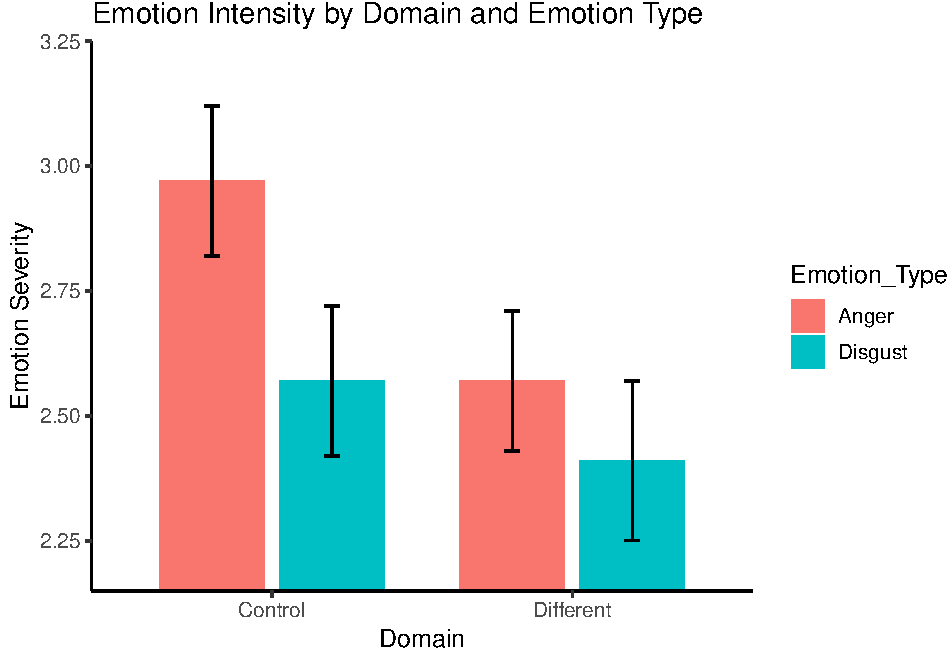
\includegraphics{APA_Report_files/figure-latex/unnamed-chunk-4-1.pdf}
\caption{\label{fig:unnamed-chunk-4}Intensity of Anger and Disgust by factor
of Domain.}
\end{figure}

\begin{table}[tbp]
\begin{center}
\begin{threeparttable}
\caption{\label{tab:anothatable}ANOVA table for Hypothesis 2}
\begin{tabular}{lllllll}
\toprule
Effect & \multicolumn{1}{c}{$F$} & \multicolumn{1}{c}{$\mathit{df}_1$} & \multicolumn{1}{c}{$\mathit{df}_2$} & \multicolumn{1}{c}{$\mathit{MSE}$} & \multicolumn{1}{c}{$p$} & \multicolumn{1}{c}{$\hat{\eta}^2_G$}\\
\midrule
Domain & 2.08 & 1 & 114 & 2.12 & .152 & .014\\
Emotion type & 7.54 & 1 & 114 & 0.59 & .007 & .014\\
Emotion type $\times$ Domain & 1.44 & 1 & 114 & 0.59 & .232 & .003\\
\bottomrule
\end{tabular}
\end{threeparttable}
\end{center}
\end{table}

A 2x2 ANOVA showed that there was a main effect of Domain (control vs
different) on Judgment, \(F(1, 114) = 17.37\), \(\mathit{MSE} = 1.11\),
\(p < .001\), \(\hat{\eta}^2_G = .102\). There was no main effect of
Judgment Type (character vs.~act) on Judgment, \(F(1, 114) = 1.05\),
\(\mathit{MSE} = 0.38\), \(p = .308\), \(\hat{\eta}^2_G = .002\).
However, there was a significant interaction effect such that Character
Judgments were more influenced by Domain than Act Judgments,
\(F(1, 114) = 25.83\), \(\mathit{MSE} = 0.38\), \(p < .001\),
\(\hat{\eta}^2_G = .054\).

A 2x2 ANOVA of Domain (control vs different) and Emotion Type (disgust
vs.~anger) showed that contrary to predictions, Domain did not have a
stronger effect on disgust than on anger, \(F(1, 114) = 1.44\),
\(\mathit{MSE} = 0.59\), \(p = .232\), \(\hat{\eta}^2_G = .003\). This
analysis also showed that anger was felt more strongly than disgust,
\(F(1, 114) = 7.54\), \(\mathit{MSE} = 0.59\), \(p = .007\),
\(\hat{\eta}^2_G = .014\). There was no main effect of Domain,
\(F(1, 114) = 2.08\), \(\mathit{MSE} = 2.12\), \(p = .152\),
\(\hat{\eta}^2_G = .014\).

A whole-sample multiple regression analysis with Character as the DV and
Disgust and Anger as the predictors was used to analyze the hypothesis
that Disgust should predict character ratings better than anger ratings.
This analysis showed that Disgust significantly predicted Character
ratings, \(b = 0.23\), 95\% CI \([0.06\), \(0.40]\), \(t(113) = 2.74\),
\(p = .007\), but anger did not, \(b = 0.14\), 95\% CI \([-0.04\),
\(0.32]\), \(t(113) = 1.50\), \(p = .137\).

A whole-sample multiple regression analysis with Act as the DV and
Disgust and Anger as the predictors was used to analyze the hypothesis
that both Disgust and Anger should predict character ratings. This
analysis showed that, as expected, Act Ratings were significantly
predicted by both disgust, \(b = 0.31\), 95\% CI \([0.18\), \(0.43]\),
\(t(113) = 4.73\), \(p < .001\), and anger, \(b = 0.22\), 95\% CI
\([0.08\), \(0.36]\), \(t(113) = 3.19\), \(p = .002\).

\subsection{Simulation-Based Power
Analysis}\label{simulation-based-power-analysis}

In this section, I model the unll-hypothesis of the 2x2 ANOVA used to
test the effect of Domain (control vs different) and Judgment Type (act
vs.~character) on judgment severity. I do this by using a
simulation-based power analysis by various effect sizes. I first
estimate the overall mean judgment, and the standard deviation of these
judgments from the data. The overall mean was 3.64, and the overall
standard deviation was 0.93.

To conduct the simulation I generate data for each subject using the
rnorm function. Each subject made a judgment of the principal's action
and character. There were 60 subjects in each Domain condition (control
vs different). For each act and character judgment, I sample 1 score
from each participant, producing 2 total scores from each participant.
To model the effect of Domain condition, I systemically increase the
mean of the Character judgments by a proportion of the standard
deviation. I use effect-sizes of 0.1, 0.2, 0.3, 0.4, 0.5, 0.6, 0.7, 0.8,
0.9, and 1; which range from small to large. For each effect-size, I run
100 simulated experiments, and save p-value for the main effect of
congruency for each simulated experiment. Then, for each effect-size, I
find the proportion of experiments that resulted in p \textless{} 0.05.
The proportion of experiments that reject the null is the power of the
design to detect an effect of each size. The simulation below finds that
this design had power of 0.90, to detect an effect of d = 0.4. It had
power of 1.00 to detect effects of d = 0.8 and larger. The full
power-curve for this design is displayed in Figure 3.

\begin{figure}
\centering
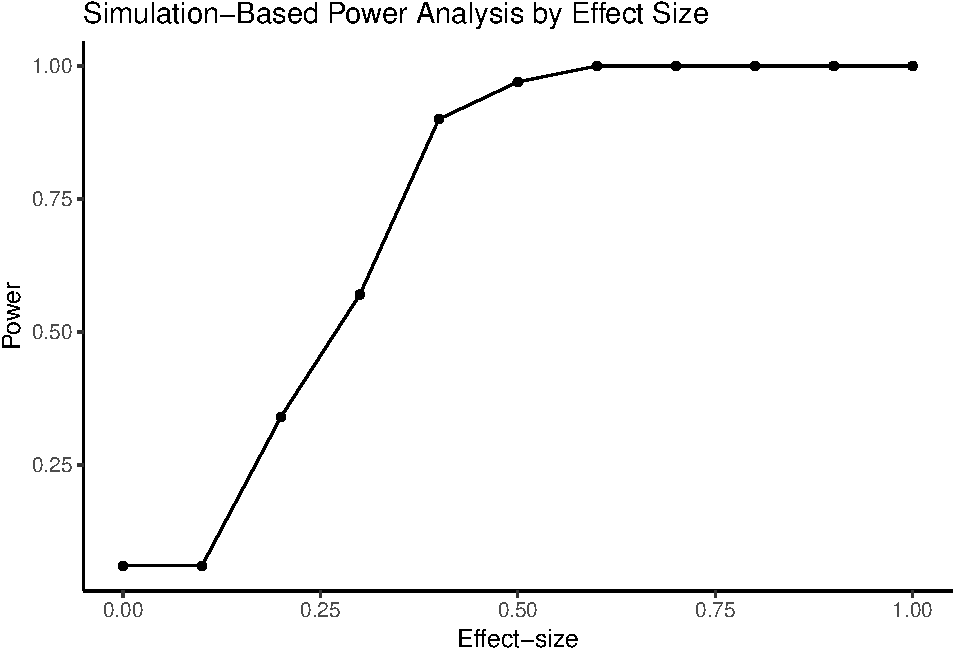
\includegraphics{APA_Report_files/figure-latex/powerfig-1.pdf}
\caption{\label{fig:powerfig}Simulation-based power curve for this design}
\end{figure}

\section{Discussion}\label{discussion}

The analyses completed in SPSS were successfully recreated using R. The
hypotheses of the experiment were generally supported, but not entirely.
The effect of Domain on Character and Act judgments did not parallel the
effect of Domain on Disgust and Anger. However, in support of our
hypotheses, only Disgust predicted Character Judgments, while both
Disgust and Anger predicted Act judgments. One possibile limitation is
that hypocrisy may not be an adequate method to manipulate bad moral
character. It might also be the case that hypocrisy increases bad moral
character but disproportionaly increases severity of a hypocratic act.

\newpage

\section{References}\label{references}

\begingroup
\setlength{\parindent}{-0.5in} \setlength{\leftskip}{0.5in}

\hypertarget{refs}{}
\hypertarget{ref-giner2017beyond}{}
Giner-Sorolla, R., \& Chapman, H. A. (2017). Beyond purity: Moral
disgust toward bad character. \emph{Psychological Science},
\emph{28}(1), 80--91.

\hypertarget{ref-uhlmann2015person}{}
Uhlmann, E. L., Pizarro, D. A., \& Diermeier, D. (2015). A
person-centered approach to moral judgment. \emph{Perspectives on
Psychological Science}, \emph{10}(1), 72--81.

\endgroup


\end{document}
